\Aufgabe{m:n-Beziehungen}

\begin{enumerate}
    \item Erstelle in YoungDB ein Datenbankmodell mit den Klassen Lehrkraft und Schulklasse, die in einer m:n-Beziehung zueinander stehen. Überlege dir sinnvolle Primärschlüssel und 1-2 Attribute und eine sinnvolle Bezeichnung für die Beziehung.
    \item Generiere nun die zugehörige Datenbank und befülle die Tabellen mit jeweils 2-3 Datensätzen.
    \item Beantworte folgende Fragen:\begin{itemize}
        \item Welchen essentiellen Unterschied gibt es zwischen m:n-Beziehungen und 1:n-/1:1-Beziehungen?\\
        \LoesungLine{Beziehungstabelle benötigt}{1}
        \item Was für Datensätze werden in der dritten Tabelle eingetragen?\\
        \LoesungLine{Paare von IDs der Datensätze der anderen Tabellen, die in Beziehung zueinander stehen}{2}
        \item Welche Spalten welcher Tabelle(n) sind Fremdschlüssel?\\\LoesungLine{beide Spalten der dritten Beziehungstabelle}{1}
        \item Welche Spalte(n) sind Primärschlüssel in der dritten Tabelle? \emph{Tipp: Was muss eindeutig sein? Probiere deine Vermutung aus, indem du versucht mehrere Datensätze mit gleichem (vermuteten) Primärschlüssel einzufügen.} 
        \\\LoesungLine{beide Spalten zusammen}{1}
        \item Ist es sinnvoll bei m:n-Beziehungen im Klassendiagramm eine Richtung anzugeben und wieso?
        \\\LoesungLine{}{2}
        \item Wie könnte man m:n-Beziehung im Klassendiagramm alternativ darstellen?
        \\\LoesungLine{zusätzliche Beziehungstabelle mit zwei 1:n-Beziehungen}{1}
        \item Zeichne die Darstellung von m:n-Beziehungen in YoungDB ein:\\\\
        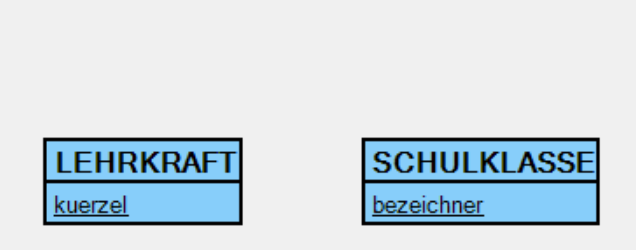
\includegraphics[width=0.6\textwidth]{Aufgaben/img/YDB_lehrerKlasse.png}
    \end{itemize}
\end{enumerate} 